\subsection{CompCert}
\begin{center}
\begin{figure}
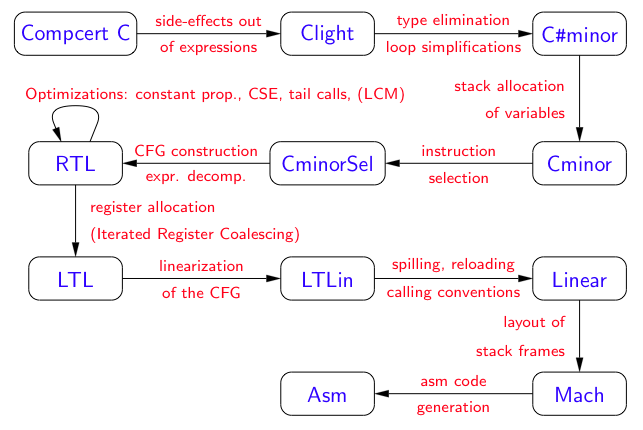
\includegraphics[scale=1]{img/passes.png}
\label{fig:compcertpasses}
\caption{Verified CompCert passes\hspace{\linewidth}S \textbf{Source: }\texttt{http://compcert.inria.fr/compcert-C.html}}
\end{figure}
\end{center}

The compiler used in this work is CompCert \cite{compcertmanual}.
It supports most of the ISO-C-99 Standard.
It can generate PowerPC, ARM and x86 assembly code.

Between the source code and the target assembly code, CompCert goes through 25 passes, including several changes of language.
The first three parse and convert the source code to CompCert C, and the last three perform printing of the assembly code, assembling and linking.
In the middle, 19 back-end passes perform various transformations, 8 of which are optimizations.
For this work, the pass from CompCert C to Clight is important, because \todo{...}.

\subsubsection{Correctness}
The parser and most of the back-end passes (see \textbf{Fig.\ref{fig:compcertpasses}.}) are verified with Coq\todo{foot note on Coq?}.
In CompCert, the behavior of a program is a trace (a list of I/O operations) and an indication on the program's termination (does it terminates? is it on an error?). %this might need better phrasing
The correctness theorem of CompCert states that the behavior of the generated code is one of the possible behaviors of the source code (C is non-deterministic). To prove it, it uses a backward simulation (see section \todo{cite section}).

\subsubsection{Optimizations}
CompCert performs the following optimizations:
Instruction selection, Common sub-expression elimination, Tail call elimination, Dead code elimination, Function inlining, Branch tuneling, Constant propagation and Register allocation \cite{compcertoverview}.
\todo{Examples the ones that will be used: DCE, DAE, CP}
 

\subsection{Memory Models}
In this section, we present the logical and concrete models with their limits, which motivates the introduction of the quasi-concrete model that has been implemented in this work.

In C semantics, the memory is divided in several \textit{memory blocks}, that contain several memory addresses. Memory blocks can be allocated (through the \texttt{malloc} function for instance), loaded, freed\dots A memory block can contain the values of several variables. 
\subsubsection{Logical Model}
The logical model described here is similar to the one used in \cite{DBLP:conf/pldi/KangHMGZV15}. However, it slightly differs from CompCert's current logical model described in \cite{leroy:hal-00703441} (see section \addref{memupdate?}).
In this model, blocks are all logical, meaning that they are not mapped to a physical memory address.
Blocks are a fixed-size array of values.
A validity flag $v$ indicates if the block has been freed.
Pointers are a pair $(l,i)$ of a block identifier and an offset inside that block.
The set $\texttt{Block}$ of blocks i defined with:
$$\texttt{Block}=\{(v,n,c)~|~v\in\texttt{Bool},n\in\mathbb{N},c\in\texttt{Val}^{n}\}$$

With a logical model, programs have infinite memory.
Moreover, a logical model can allow functions to have exclusive control over a logical block.
When a block identifier does not escape when calling a function (\textit{i.e.} if the block identifier cannot be found inside the global variables or the function arguments), then the called function cannot access the block \addref{section memupdate on abstract analysis?}.% too long sentence?
This allow for many optimizations. \todo{example}.

However, logical models do not support integer-pointer casts. They can allow some arithmetic operations on offsets, but is impossible to get a physical address from a block.

\subsubsection{Concrete Model}
The concrete model aims to reflect the memory of a real machine.
The memory itself is a $2^{32}$-sized array of values, and \texttt{Allocated}, a list of allocated blocks.
Blocks are simply a pair of a concrete address and a size.
$$\texttt{Block}=\{(p,n)~|~p\in\texttt{int32},n\in\texttt{int32}\}$$
The concrete memory should require from the allocated blocks to be consistent:
$$\textit{No overflow:}\quad\forall (p,n)\in\texttt{Allocated}, [p,p+n]\subseteq]0,2^{32}[$$
$$\textit{No overlap:}\quad\forall (p_1,n_1), (p_2,n_2)\in\texttt{Allocated}, [p_1,n_1]\text{ and }[p_2,n_2]\text{ are disjoint.}$$
In the concrete model, integer-pointer cast is possible because concrete addresses are already integer values.

However, optimizations such as constant propagation and dead allocation elimination are not supported in many cases, because external functions might change the value of any address. In the concrete model, there is no ownership notion, and every address is always accessible.
\subsubsection{Quasi-concrete model}
In \cite{DBLP:conf/pldi/KangHMGZV15}, a new memory model is presented. The motivation is to have a memory model which allows integer-pointer casting, but still supports common optimizations.
This is achieved with the following definitions.
A block can be either logical or concrete, in which case it has a concrete address. This is represented by the value $p$.
$$\texttt{Block}=\{(v,p,n,c)~|~v\in\texttt{Bool},n\in\mathbb{N},c\in\texttt{Val}^{n},p\in\texttt{int32}\cup\{\undef\}\}$$
The concrete blocks need to be consistent:
$$\textit{No overflow:}\quad\forall (v,p,n,c)\in\texttt{Blocks}, (p\neq\undef~\wedge~ v=\textit{true})\implies[p,p+n]\subseteq]0,2^{32}[$$
$$\textit{No overlap:}\quad\forall (p_1,n_1), (p_2,n_2)\in\texttt{Blocks}, (p_1\neq\undef~\wedge~p_2\neq\undef ~\wedge~ v_1=v_2=\textit{true})\implies [p_1,n_1]\text{ and }[p_2,n_2]\text{ are disjoint.}$$
A pointer is a pair $(l,i)$ of a block identifier and an offset inside that block. If the block $l$ starts at the address $p\neq\undef$, then $(l,i)$ can be cast as the integer $p+i$ and vice versa (thanks to the property of no overlapping, an integer can correspond to at most one valid concrete block).

Optimizations are still be possible with logical blocks, because they do not have concrete addresses, and integer-pointer casts are possible with concrete blocks.
To allow as many optimizations as possible, we should use as many logical blocks as possible. Thus, new blocks should be made logical when allocated.
However, for each pointer to integer cast, we need a concrete block. Then we transform each pointer to integer cast by adding a \textit{capture} function just before it. This function transforms a logical block into a concrete one, giving it a concrete address that still satisfy the memory consistency. Its semantics are described section \addref{section sem}.
It introduces non-determinism in every language of CompCert (including the assembly). This is handled in section \addref{section mixedsim}.

The quasi-concrete is described in many details in \cite{DBLP:conf/pldi/KangHMGZV15}.
\subsubsection{Optimization and casts examples}
...
\todo{examples of optimizations and casts for the 3 models}
\todo{explain what is assumed when doing optimizations: one cannot guess an address}

\subsection{Simulations}
\todo{Maybe this will be moved to section mixedsim}




